\documentclass[border=10pt]{standalone}
\usepackage{underscore}
\usepackage{tikz}
\usetikzlibrary{shapes,arrows,positioning,calc,backgrounds,matrix,fit,decorations.pathreplacing}

\newcount\index
\newcommand{\diaName}{default name}
\newcommand{\diaWidth}{10em}
\newcommand{\diaHeight}{2em}
\newcommand{\updateIndex}{\advance\index by 1\relax}
\newcommand{\lastId}{\diaName-\the\numexpr\index-1\relax}
\newcommand{\id}{\diaName-\the\index}

\newcommand{\record}[2]{
    \node[fixed node={\diaWidth}{\diaHeight},below=of \lastId,#1](\id){#2};
    \updateIndex
}
%%% environment struct
\newenvironment{struct}[3]
{
    \index=0
    \renewcommand{\diaName}{#1}
    \renewcommand{\diaWidth}{#2}
    \renewcommand{\diaHeight}{#3}
}
{
    \node[fit=(\diaName-0)(\lastId),inner sep=0pt](\diaName){};
}
%%% environment struct end


\tikzset{
    table/.style 2 args={
        draw,
        rectangle,
        inner sep=0pt,
        matrix of nodes,
        nodes in empty cells,
        nodes={
            draw,
            font=\ttfamily,
            align=center,
            text width=#1,
            outer sep=0pt,
            inner sep=0.3em,
            minimum height=1.6em
        },
        label={[align=center]90:\bf{#2}}
    },
    table/.default={10cm}{},
    right brace/.style 2 args={
        decorate,
        decoration={brace,amplitude=#1,raise=#2}
    },
    right brace/.default={8pt}{2pt},
    right note/.style={right=#1},
    right note/.default={0.3cm},
    left note/.style={left=#1},
    left note/.default={0.3cm},
    left brace/.style 2 args={
        decorate,
        decoration={brace,amplitude=#1,raise=#2,mirror}
    },
    left brace/.default={8pt}{2pt},
    right addr note/.style={right=#1},
    right addr note/.default={0.5cm},
    left addr note/.style={left=#1},
    left addr note/.default={0.5cm},
    arrow/.style={>=stealth',->},
    fixed node/.style 2 args={
        node distance=0,
        outer sep=0,
        inner sep=0,
        draw,
        font=\ttfamily,
        rectangle,
        minimum width=#1,
        minimum height=#2
    },
    title node/.style={rectangle,inner sep=1em},
    blank cell/.style={fill=white,minimum height=1cm},
    non blank cell/.style={fill=cyan!30,minimum height=#1}
}


\newcommand{\sybwd}{32em}
\newcommand{\sybht}{2em}
\newcommand{\sybleftwd}{12em}
\newcommand{\sybleftht}{5em}
\newcommand{\sybrightwd}{20em}
\newcommand{\sybrightht}{2em}

\newcommand{\methodwd}{36em}
\newcommand{\methodht}{2em}
\newcommand{\methodleftwd}{20em}
\newcommand{\methodleftht}{3em}
\newcommand{\methodrightwd}{16em}
\newcommand{\methodrightht}{4em}

\begin{document}
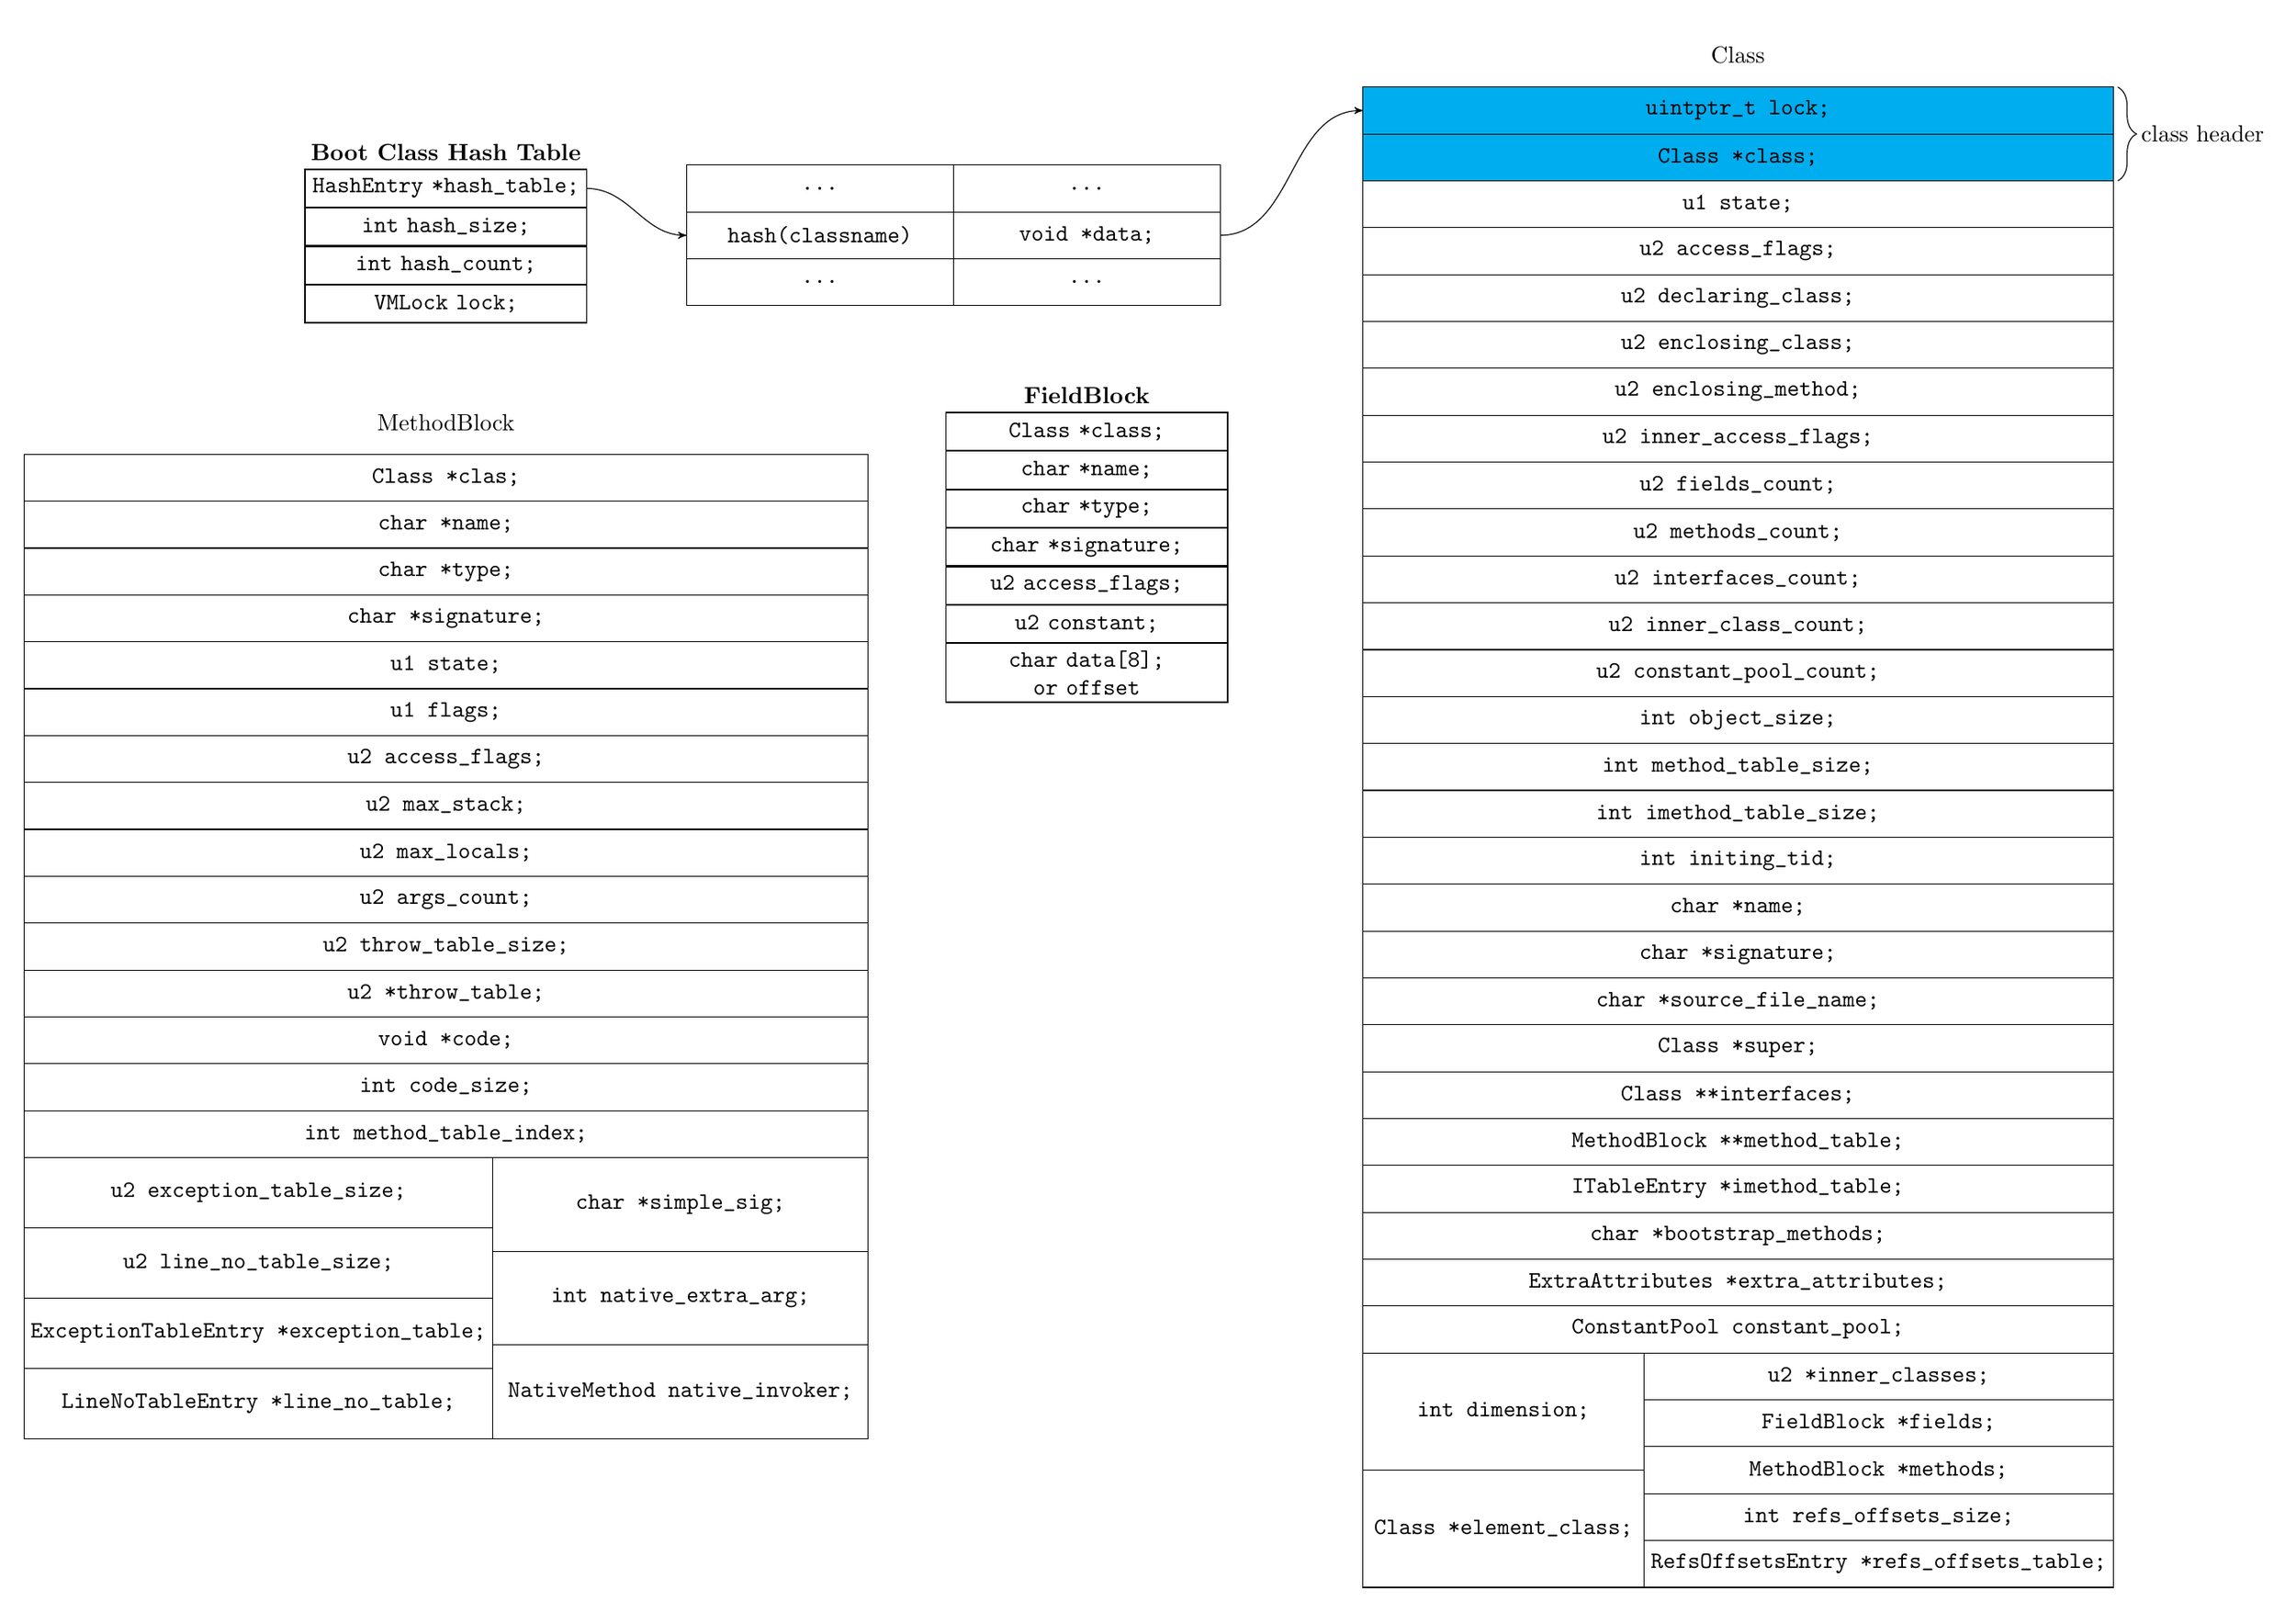
\begin{tikzpicture}

    %%% hashtable
    \matrix (hashtable) [table={4cm}{Boot Class Hash Table}] {
      ||{HashEntry *hash\_table;}\\
      ||{int hash\_size;}\\
      ||{int hash\_count;}\\
      ||{VMLock lock;}\\
    };
    
    
    %%% hash data
    \node[fixed node={4cm}{2em}, right=of hashtable-1-1, xshift=1.5cm](data){...};
    \node[fixed node={4cm}{2em}, below=of data](data01){hash(classname)};
    \node[fixed node={4cm}{2em}, below=of data01](data02){...};
    \node[fixed node={4cm}{2em}, anchor=north west,](data1) at(data.north east){...};
    \node[fixed node={4cm}{2em}, below=of data1](data11){void *data;};
    \node[fixed node={4cm}{2em}, below=of data11](data12){...};


    %%% Class
    \node[rectangle,inner sep=1em,right=5cm of data1, xshift=2cm, yshift=2cm](title){Class};
    \node[fixed node={\sybwd}{\sybht},fill=cyan,below=of title](a0){uintptr\_t lock;};
    \node[fixed node={\sybwd}{\sybht},fill=cyan,below=of a0](a1){Class *class;};
    \node[fixed node={\sybwd}{\sybht},below=of a1](a2){u1 state;};
    \node[fixed node={\sybwd}{\sybht},below=of a2](a3){u2 access\_flags;};
    \node[fixed node={\sybwd}{\sybht},below=of a3](a4){u2 declaring\_class;};
    \node[fixed node={\sybwd}{\sybht},below=of a4](a5){u2 enclosing\_class;};
    \node[fixed node={\sybwd}{\sybht},below=of a5](a6){u2 enclosing\_method;};
    \node[fixed node={\sybwd}{\sybht},below=of a6](a7){u2 inner\_access\_flags;};
    \node[fixed node={\sybwd}{\sybht},below=of a7](a8){u2 fields\_count;};
    \node[fixed node={\sybwd}{\sybht},below=of a8](a9){u2 methods\_count;};
    \node[fixed node={\sybwd}{\sybht},below=of a9](a10){u2 interfaces\_count;};
    \node[fixed node={\sybwd}{\sybht},below=of a10](a11){u2 inner\_class\_count;};
    \node[fixed node={\sybwd}{\sybht},below=of a11](a12){u2 constant\_pool\_count;};
    \node[fixed node={\sybwd}{\sybht},below=of a12](a13){int object\_size;};
    \node[fixed node={\sybwd}{\sybht},below=of a13](a14){int method\_table\_size;};
    \node[fixed node={\sybwd}{\sybht},below=of a14](a15){int imethod\_table\_size;};
    \node[fixed node={\sybwd}{\sybht},below=of a15](a16){int initing\_tid;};
    \node[fixed node={\sybwd}{\sybht},below=of a16](a17){char *name;};
    \node[fixed node={\sybwd}{\sybht},below=of a17](a18){char *signature;};
    \node[fixed node={\sybwd}{\sybht},below=of a18](a19){char *source\_file\_name;};
    \node[fixed node={\sybwd}{\sybht},below=of a19](a20){Class *super;};
    \node[fixed node={\sybwd}{\sybht},below=of a20](a21){Class **interfaces;};
    \node[fixed node={\sybwd}{\sybht},below=of a21](a22){MethodBlock **method\_table;};
    \node[fixed node={\sybwd}{\sybht},below=of a22](a23){ITableEntry *imethod\_table;};
    \node[fixed node={\sybwd}{\sybht},below=of a23](a24){char *bootstrap\_methods;};
    \node[fixed node={\sybwd}{\sybht},below=of a24](a25){ExtraAttributes *extra\_attributes;};
    \node[fixed node={\sybwd}{\sybht},below=of a25](a26){ConstantPool constant\_pool;};
    
    \node[fixed node={\sybleftwd}{\sybleftht},anchor=north west](a100) at (a26.south west){int dimension;};
    \node[fixed node={\sybleftwd}{\sybleftht},below=of a100]    (a101){Class *element\_class;};
    
    \node[fixed node={\sybrightwd}{\sybrightht},anchor=north west]      (a200) at (a100.north east){u2 *inner\_classes;};
    \node[fixed node={\sybrightwd}{\sybrightht},below=of a200]          (a201){FieldBlock *fields;};
    \node[fixed node={\sybrightwd}{\sybrightht},below=of a201]          (a202){MethodBlock *methods;};
    \node[fixed node={\sybrightwd}{\sybrightht},below=of a202]          (a203){int refs\_offsets\_size;};
    \node[fixed node={\sybrightwd}{\sybrightht},below=of a203]          (a204){RefsOffsetsEntry *refs\_offsets\_table;};
    

    %%% Field
    \matrix (fieldblock) [table={4cm}{FieldBlock},below=3cm of data,xshift=4cm] {
        ||{Class *class;}\\
        ||{char *name;}\\
        ||{char *type;}\\
        ||{char *signature;}\\
        ||{u2 access\_flags;}\\
        ||{u2 constant;}\\
        ||{char data[8]; or offset}\\
    };


    %%% MethodBlock
    \node[rectangle,inner sep=1em,below=1cm of hashtable](method title){MethodBlock};
    \node[fixed node={\methodwd}{\methodht},below=of method title](m1){Class *clas;};
    \node[fixed node={\methodwd}{\methodht},below=of m1](m2){char *name;};
    \node[fixed node={\methodwd}{\methodht},below=of m2](m3){char *type;};
    \node[fixed node={\methodwd}{\methodht},below=of m3](m4){char *signature;};
    \node[fixed node={\methodwd}{\methodht},below=of m4](m5){u1 state;};
    \node[fixed node={\methodwd}{\methodht},below=of m5](m6){u1 flags;};
    \node[fixed node={\methodwd}{\methodht},below=of m6](m7){u2 access\_flags;};
    \node[fixed node={\methodwd}{\methodht},below=of m7](m8){u2 max\_stack;};
    \node[fixed node={\methodwd}{\methodht},below=of m8](m9){u2 max\_locals;};
    \node[fixed node={\methodwd}{\methodht},below=of m9](m10){u2 args\_count;};
    \node[fixed node={\methodwd}{\methodht},below=of m10](m11){u2 throw\_table\_size;};
    \node[fixed node={\methodwd}{\methodht},below=of m11](m12){u2 *throw\_table;};
    \node[fixed node={\methodwd}{\methodht},below=of m12](m13){void *code;};
    \node[fixed node={\methodwd}{\methodht},below=of m13](m14){int code\_size;};
    \node[fixed node={\methodwd}{\methodht},below=of m14](m99){int method\_table\_index;};

    \node[fixed node={\methodleftwd}{\methodleftht},anchor=north west] (m100) at (m99.south west) {u2 exception\_table\_size;};
    \node[fixed node={\methodleftwd}{\methodleftht},below=of m100](m101){u2 line\_no\_table\_size;};
    \node[fixed node={\methodleftwd}{\methodleftht},below=of m101](m102){ExceptionTableEntry *exception\_table;};
    \node[fixed node={\methodleftwd}{\methodleftht},below=of m102](m103){LineNoTableEntry *line\_no\_table;};

    \node[fixed node={\methodrightwd}{\methodrightht},anchor=north west](m200) at (m100.north east) {char *simple\_sig;};
    \node[fixed node={\methodrightwd}{\methodrightht},below=of m200](m201){int native\_extra\_arg;};
    \node[fixed node={\methodrightwd}{\methodrightht},below=of m201](m202){NativeMethod native\_invoker;};

    %%% lines
    \draw[arrow] (hashtable-1-1.east) to[out=0,in=180] (data01.west);
    \draw[arrow] (data11.east) to[out=0,in=180] (a0.west);
    \draw[right brace] (a0.north east) -- node[right note]{class header} (a1.south east);
\end{tikzpicture}
\end{document}


